\chapter{Alignment of the SciFi}
\label{sec:story}

For the upgrade the LHCb detector was completely rebuilt. In place of the previous IT and OT a new tracking detector was built which utilizes scintillating fibre called SciFi Tracker. The front-end electronics were also upgraded to handle the increasing data rate. For the new SciFi Tracker a new software is used.

Because of the introduction of the new software, the alignment configuration needs to be determined from the beginning. The goal is to find a configuration that can accurately reproduce the position of the real detector and can correct for ``weak modes''.
With some alignment parameters being highly correlated, detector components may move in the same direction or by the same amount. This is called a ``weak mode''. The movements do not affect the alignment $\chi^2$ since the residuals have not changed. Results of weak modes are biases in track parameters and poor alignment convergence.
One of the most visible weak modes is the curvature bias. There a different ways to reduce the effect of weak modes for example using an overlapping detector design or using different data sets to gather more information.

\section{Alignment Configuration}

An alignment configuration is a specific selection of detector elements, alignment parameters, constraints and track- and vertex-selections used for the alignment.
Alignment parameters are the specific degrees of freedom used for the alignment and for each detector element. The Alignment parameters can be any combination of translations and rotations around the $x$, $y$ and $z$ axis($Tx$, $Ty$, $Tz$, $Rx$, $Ry$, $Rz$).
The configuration that produces the best estimate for the detector position is the best candidate and will be used for the Run 3 data taking.
A track and vertex reconstruction is performed before the alignment is evaluated. Depending on the tracks used the output can be different. Mainly two different track selections will be used throughout the thesis shown in table \ref{tab:tracks}

\begin{table}[!ht]
    \centering
    \begin{tabular}{c|c}
        \toprule
            Tracks & Selections \\
        \midrule
            GoodLongTracks &  $P_{\text{total, min}} = \SI{5000}{\mega\electronvolt}$ \\
            & $P_{\text{total, max}} = \SI{200000}{\mega\electronvolt}$ \\
            & $p_\text{T, min} = \SI{200}{\mega\electronvolt}$ \\
            & maximum $\chi^2 = 5$ \\
            & "long" track type \\
            \hline
            HighMomentumTTracks & $P_{\text{total, min}} = \SI{50000}{\mega\electronvolt}$ \\
            & maximum $\chi^2 = 5$ \\
            & "TTrack" track type \\
        \bottomrule
    \end{tabular}
    \caption{SciFi track selection.}
    \label{tab:tracks}
\end{table}

The alignment runs were performed with alignment specific packages from Alignment/Escher and Alignment/TAlignment\cite{align}.
During the alignment, Lagrange constraints can be utilized to minimize alignment
parameter $\alpha $ under the condition
\begin{equation}
  f(\alpha) = 0
\end{equation}
and adding the Lagrange parameter $\lambda$ to get
\begin{equation}
  \Delta \chi^2 = \lambda f(\alpha)\,.
\end{equation}
Lagrange constraints are added to fix loosely constrained degrees of freedom and can be used for any linear combination of translations and rotations as shown in table \ref{tab:lagr}

\begin{table}[!ht]
    \centering
    \begin{tabular}{c|c}
        \toprule
            Tx, Ty, Tz & translation in x, y, z \\
            Rx, Ry, Rz & rotation around x, y, z \\
            Szx, Szy & shearing of x and y along z \\
            Szz, Sxx & scaling in x and z \\
        \bottomrule
    \end{tabular}
    \caption{Lagrange constraints that can be used as alignment parameters.}
    \label{tab:lagr}
\end{table}

An illustration of shearing is shown in figure \ref{fig:shear}.

\begin{figure}
    \centering
    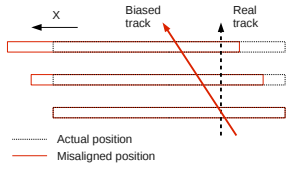
\includegraphics[width=0.6\textwidth]{plots/shearing.png}
    \caption{An illustration of shearing.}
    \label{fig:shear}
\end{figure}

In the software, a Langrange constraint is defined by three elements. A name which can be chosen by the user, the detector element and the alignment parameters, seperated by a colon.

The starting constraints are defined as the following table \ref{tab:cond}, which are based on the alignment conditions from the OT and knowledge from experts.
\begin{table}[!ht]
    \centering
    \begin{tabular}{c | c | c}
        \toprule
            element & positions & uncertainties \\
        \midrule
            $\text{FT}$ & 0 0 0 0 0 0 & 1 1 1 0.0003 0.0003 0.0003 \\
            $\text{FT/T.}$ & 0 0 0 0 0 0 & 1 1 1 0.0003 0.0003 0.0003 \\
            $\text{FT/T./Layer(X1|U|V|X2)}$ & 0 0 0 0 0 0 & 0.2 0.2 0.2 0.0001 0.0001 0.0001 \\
            $\text{FT/.*Module.}$ & 0 0 0 0 0 0 & 0.1 0.1 0.1 0.001 0.001 0.001 \\
            $\text{FT/.*Mat.}$ & 0 0 0 0 0 0 & 0.05 0.05 0.05 0.1 0.1 0.1 \\
        \bottomrule
    \end{tabular}
    \caption{starting condition of the SciFi Tracker.}
    \label{tab:cond}
\end{table}

The SciFi Tracker is referred to as Forward Tracker (FT) in the software.
The first element in each row of the starting conditions is the detector element.
The first set of six numbers are hardcoded parameters for each of the three translation degrees of freedom and three rotational degrees of freedom (Tx, Ty, Tz, Rx, Ry, Rz). They are set to be zero to match the known position of the detector in the Monte Carlo Simulation (MC).
and the second set of six parameters are the corresponding uncertainties.
The scale for the translations are $\si{\milli\metre}$ and the scale for the rotations being $\si{\radian}$. A survey uncertainty of $\num{0.0001}$ stands for $\SI{0.1}{\milli\radian}$.
During this thesis, the LHC beam was off and the SciFi detector was still being constructed. The alignment tests in this thesis use Monte Carlo simulated data to test the alignment software for the SciFi.

\section{Null tests and software tests}
\subsection{Software configurations and samples}
\begin{figure}
  \centering
  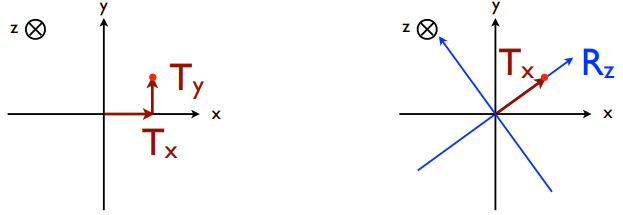
\includegraphics[width=0.75\textwidth]{plots/point_dofs.png}
  \caption{Different ways of describing a measurement point inside the detector(draw this again).}
  \label{fig:dofs}
\end{figure}

At first, a series of tests regarding different degrees of freedom and Lagrange constraints is performed to find the optimal solution for the SciFi Tracker.

The detector layers in the MC are all centered around the beam pipe with no shifting in any direction and the goal is to align the real detector layers to mirror the layers in the software and reduce the shifting as close to zero as possible.

Figure \ref{fig:dofs} is used to demonstrate which degrees of freedom can be used
to describe a point in the detector or a shift in coordinates.
On the left-hand side the measurement point is described through cartesian coordinates and on the right-hand side it is described via polar coordinates.

Problems with the shearing constraints were seen in the VELO alignment, so that a similar analysis for the SciFi was considered.
The parameters used for the VELO were changed to fit the SciFi Tracker and resulted in the following configuration:

\begin{lstlisting}[language=Python]
    dofs = "TxTzRxRz"
    elements.FTStations(dofs)
    elements.FTFrameLayers(dofs)
    TrackSelections = GoodLongTracks()
\end{lstlisting}

The dataset\footnote{upgrade\_DC19\_01\_MinBiasMU} used taken from the TestFileDB\cite{testDB} and will be used for the upcoming tests until a different set is mentioned.
As the DoFs, x- and z-translation as well as rotations around the x- and z-axis are used and are the only relevant DoFs for the alignment since y-translation and rotations around the y-axis can be constructed from the other degrees of freedom.
For the alignment runs, ten iterations were used and is not using input misalignment, so a perfectly aligned detector is expected from the MC.
The alignment constants after each iteration are passed on to the next iteration.
Convergence of the alignment is defined by the difference between the variation of the alignment parameters of the current iteration to the last iteration. If the variation is sufficiently small, the alignment is converged.
The alignable objects are the (T-)stations and the frame layers within a station and the track selection is chosen to be \textit{GoodLongTracks} as a starting point. This will be called \textit{baseline} or \textit{baseline configuration}.
The baseline is unconstrained in order to check the accuracy of the alignment software without constraints and look for weak modes.
The baseline is completely unconstrained.
The frame layers, also called half layers, are divided into two quarters which are the top half and bottom half of the frame layer.

\subsection{Aligning with translations and constraints}
The first configuration tested against the baseline is called “noRotation”. Comparisons of this configuration with the baseline are shown in figure \ref{fig:june_2} and figure \ref{fig:june_2_1}, for 1000 and 7000 simulated events respectively.

In these plots, the measurement points are the mean position of each layer, and the errorbars are root-mean-square errors (RMS) and come from the difference between the C-side and the A-side of the detector layer and is not the measurement uncertainty.
The group position is the global position of the stations and layers inside the LHCb experiment, where $z = 0$ is the far left side of the experiment where the VELO begins.

The "noRotation" configuration is defined as:

\begin{lstlisting}[language=Python]
    dofs = "TxTz"
    elements.FTStations(dofs)
    elements.FTFramelayers(dofs)
    TrackSelections = GoodLongTracks()
    constraints = [
        "station1 : FT/T1 : Tx Tz",
        "station2 : FT/T2 : Tx Tz",
        "station3 : FT/T3 : Tx Tz",
        "frontCSide : FT/T3/Layer(X1|U)/Quarter(0|2) : Tx Tz",
        "backCSide  : FT/T3/Layer(V|X2)/Quarter(0|2) : Tx Tz",
        "frontASide : FT/T3/Layer(X1|U)/Quarter(1|3) : Tx Tz",
        "backASide  : FT/T3/Layer(V|X2)/Quarter(1|3) : Tx Tz"
    ]
\end{lstlisting}

The first three constraints on all stations regarding translations brings the movement of the frame layers within a station to around zero which can be seen clearly in figure\ref{fig:june_2}. The last four constraints restrict the sum of the movement of the half-layers inside each C-frame to be zero, which brings the x translation of the half-layers in station three even closer to zero.
Even though the alignment improved the amount of constraints cannot recover from potential misalignments because the constraints hinder the stations from moving.

In an ideal alignment we want as few constraints as possible so that the alignable objects can be aligned and converge towards the optimal position based on the track reconstruction.
In this measurement 3000 events were used. The associated graphs for $Tx$ plotted against the group position in $z$ are shown in figure \ref{fig:june_2}.

A prominent problem visible is the layer separation between the X-layers and the stereo layers as well as a separation between the C-frames inside each station.

\begin{figure}
  \centering
  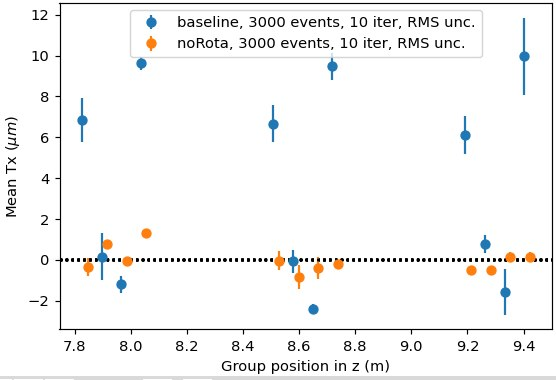
\includegraphics[width=0.9\textwidth]{plots/renewed_plots/lxplus/4_3.jpeg}
  \caption{comparison of different configurations without rotational constraints in every station, magnet up and 3000 events. plotted is translation in $x$ versus global $z$.}
  \label{fig:june_2}
\end{figure}

\begin{figure}
  \centering
  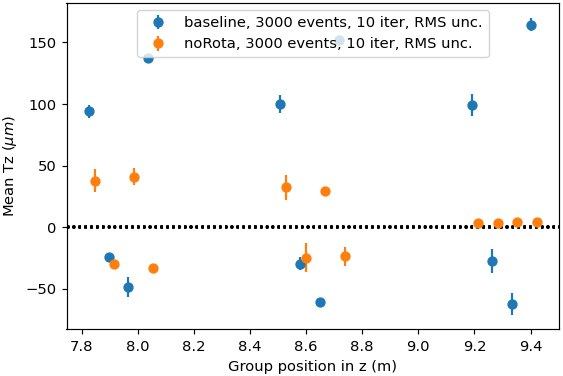
\includegraphics[width=0.9\textwidth]{plots/renewed_plots/lxplus/4_4.jpeg}
  \caption{comparison of different configurations without rotational constraints in all stations, magnet up and 3000 events. plotted is $z$ translation versus global $z$.}
  \label{fig:june_2_1}
\end{figure}

In figure \ref{fig:june_2_1} the $z$-translation is plotted against the group position in $z$. In comparison to \ref{fig:june_2} an overall improvement of the baseline is visible and the layer-splitting is reduced but still prominent. The green measurement shows no direct improvement since the layers are already pretty close to zero in x-direction.
Using 7000 events instead of 1000 events showed a more realistic picture but
took more time to compute especially for 10 alignment iterations.
For the following configuration, 3000 simulated events were used to shorten the computing time while still yielding an accurate representation of the situation.

% for comparisons include the 3000MU plot from renewed_plots
\subsection{Aligning with translations, rotations, and constraints}
The next configuration tested will be called "half C-frame". This configuration is defined as

\begin{lstlisting}[language=Python]
    dofs = "TxTzRxRz"
    elements.FTStations(dofs)
    elements.FTFramelayers(dofs)
    TrackSelections = GoodLongTracks()
    constraints = [
        "station1 : FT/T1 : Tx Tz",
        "station2 : FT/T2 : Tx Tz",
        "station3 : FT/T3 : Tx Tz",
        "frontCSide : FT/T3/Layer(X1|U)/Quarter(0|2) : Tx Tz : total",
        "backCSide  : FT/T3/Layer(V|X2)/Quarter(0|2) : Tx Tz : total"
]
\end{lstlisting}

The degrees of freedom used for this configuration are the same as in the baseline configuration for the same reason.
We chose to align the stations in the given DoFs to fix their overall position in the SciFi and also align the half-layers since we see a separation between the layers which we want to correct with the following constraints.
The stations are constrained in $Tx$ and $Tz$ to fix the overall movement inside the SciFi. The second to last constraint (``frontCSide´´) is constraining the first to half-layers in station three in their total movement along the x- and z-axis.
The last constraint works the same but for the back two half-layers of station three.

and the comparison to the baseline is shown in figure \ref{fig:june_3}.
Here the stations and layers are aligned in $Tx$, $Tz$, $Rx$ and $Rz$ but the stations are still only constrained in their translations. Also, the last station only has one side of each C-frame constrained. The additional keyword \textbf{total} constraints
the difference of the quarters to zero with respect to the nominal position. As seen in figure \ref{fig:june_3} the first two layers have an average position of zero but the individual position is not. The same is seen in the last two layers of each station.

This new configuration in orange converged after 12 iterations as seen in figure \ref{fig:conv}.
This figure shows the mean of the modules in each station per iteration. The modules of station one are the (colour1) dots, the modules for station two are coloured (colour2) and for station three is coloured (colour3).
The horizontal red line is the nominal position of the SciFi in MC, where the aligned detector should be.
The blue, dotted, vertical line marks the point of convergence for the alignment run.
Normally, an alignment job should converge after three to five iterations. If the convergence happens later there could be a problem with the constraints which prevent the alignment from converging because they are implemented wrongly, are redundant or weak modes hinder the convergence.

\begin{figure}
  \centering
  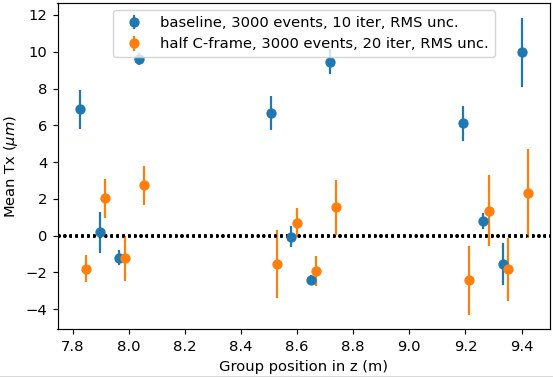
\includegraphics[width=0.9\textwidth]{plots/renewed_plots/lxplus/4_5.jpeg}
  \caption{analysed 20 iterations for $x$ translation behavior for configuration "half C-frame" plotted against the baseline configuration.}
  \label{fig:june_3}
\end{figure}

\begin{figure}
  \centering
  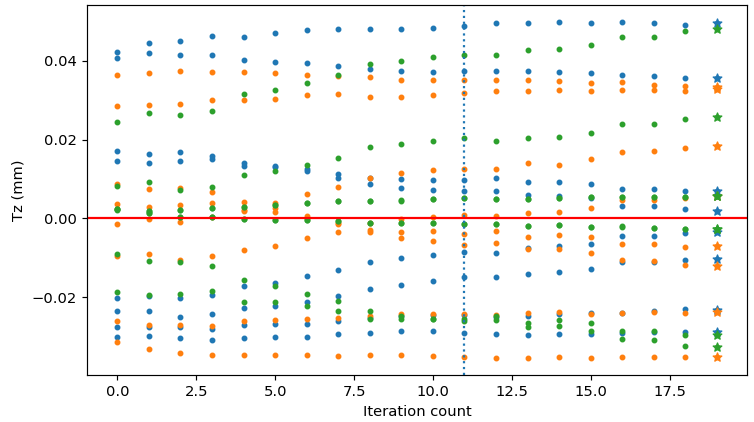
\includegraphics[width=0.9\textwidth]{plots/scatter_fig_4_4_convergence.png}
  \caption{convergence of the alignment after 12 iterations from configuration "half C-frame".}
  \label{fig:conv}
\end{figure}

\section{Null tests with rotational constraints}
In the previous section rotations were not used inside the constraints. Now the constraints will include rotational constraints and test the changes.

Similar to the "noRotation" configuration the same constraints were used but for different degrees of freedom. The new configuration is called "Full DoF" which uses every degree of freedom and is defined as:

\begin{lstlisting}[language=Python]
    dofs = "TxTyTzRxRyRz"
    elements.FTStations(dofs)
    elements.FTFramelayers(dofs)
    TrackSelections = GoodLongTracks()
    constraints = [
        "station1 : FT/T1 : Tx Ty Tz Rx Ry Rz",
        "station2 : FT/T2 : Tx Ty Tz Rx Ry Rz",
        "station3 : FT/T3 : Tx Ty Tz Rx Ry Rz",
        "frontCSide : FT/T3/Layer(X1|U)/Quarter(0|2) : Tx Ty Tz Rx Ry Rz",
        "backCSide  : FT/T3/Layer(V|X2)/Quarter(0|2) : Tx Ty Tz Rx Ry Rz",
        "frontASide : FT/T3/Layer(X1|U)/Quarter(1|3) : Tx Ty Tz Rx Ry Rz",
        "backASide  : FT/T3/Layer(V|X2)/Quarter(1|3) : Tx Ty Tz Rx Ry Rz"
        ]
\end{lstlisting}

In figure \ref{fig:june_4} x-translation and z-translation with regards to the group position are shown.

\begin{figure}
  \centering
  \begin{subfigure}[b]{0.7\textwidth}
    \centering
    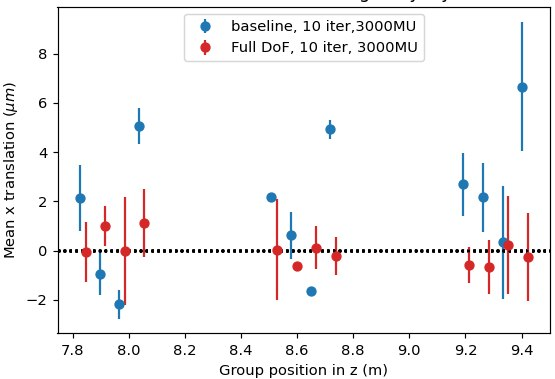
\includegraphics[width=\textwidth]{plots/renewed_plots/lxplus/4_7_a.jpeg}
    \caption{x-translation versus group position in z.}
    \label{fig:june_4_1}
  \end{subfigure}
  \hfill
  \begin{subfigure}[b]{0.7\textwidth}
    \centering
    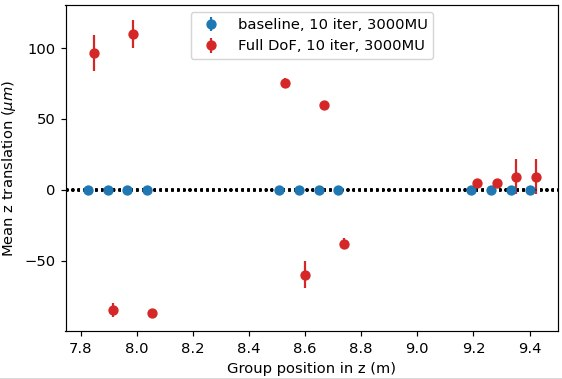
\includegraphics[width=\textwidth]{plots/renewed_plots/lxplus/4_7_b.jpeg}
    \caption{z-translation versus group position in z.}
    \label{fig:june_4_2}
  \end{subfigure}
  \caption{"Full DoF" configuration (red) plotted versus baseline configuration (blue) for 3000 events.}
  \label{fig:june_4}
\end{figure}

Figure \ref{fig:june_4_1} still shows layer separation in station 1 more similar to figure \ref{fig:june_3} than to figure \ref{fig:june_2_1}.
Since the constraints are the same and the amount of degrees of freedoms increased,
it is visible that using more DoFs makes the alignment worse. Therefore the degrees of freedom must be chosen wisely.

Regarding the z-translation the plot is only shown to demonstrate the large separation of layers. the baseline was not aligned in $Tz$ so there is no comparison.

The RMS uncertainty on the measurements is a result of the separation between A-side and C-side. For configuration "Full DoF", a plot showing the C-side and A-side difference in x-translation is presented in figure \ref{fig:june_5} and for z-translation in figure \ref{fig:june_6}.

A clear layer separation is visible in terms of layer translation along the beam pipe\ref{fig:june_5}.
The first and third layer in each station move away from the IP and the second and
fourth layer move towards the IP.
Because of the many constraints that are applied to T3, the RMS uncertainty in the other stations get worse. Because the last station is overconstrained the track reconstruction moves the other stations accordingly which results in a larger RMS uncertainty for the half-layers in station 1 and 2.

\begin{figure}
  \centering
  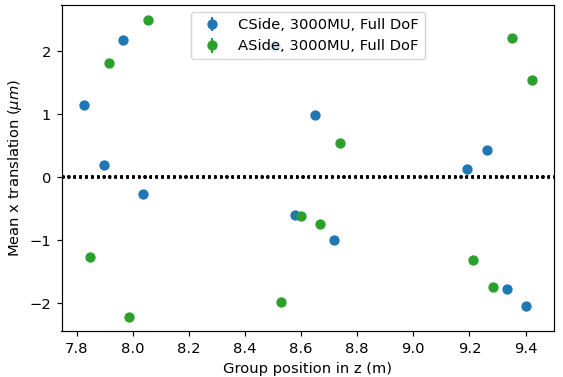
\includegraphics[width=0.8\textwidth]{plots/renewed_plots/CA_allT_halfT3_Tx.png}
  \caption{compare C-Side to A-Side for translation in x direction.}
  \label{fig:june_5}
\end{figure}

\begin{figure}
  \centering
  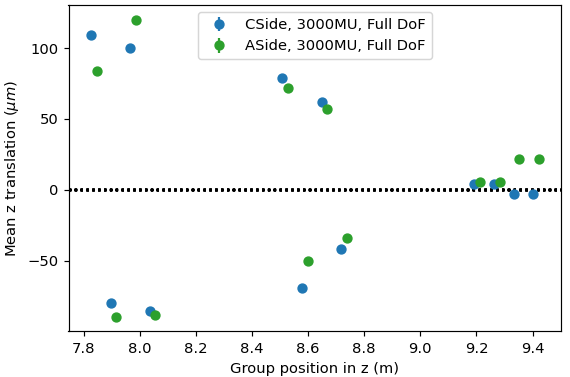
\includegraphics[width=0.8\textwidth]{plots/renewed_plots/CA_allT_halfT3_Tz.png}
  \caption{compare C-Side to A-Side for translation in z direction.}
  \label{fig:june_6}
\end{figure}

The x-translation in Figure \ref{fig:june_5} also shows some separation, the last two layers in station 3 are separated from the first two regarding z-translation. Especially the half-layers in the last station should be fixed around zero with the constraints added. The sum of all translations should be zero with each individual layer movement being small.

This result is unexpected with the constraints added. In the next sections, more tests are described, while the underlying cause of these unexpected results is described in Section \ref{sec:clusterbias}.

\subsection{Checking rotational degrees of freedom}
\label{sec:test_and_c5}
The Next configuration tested is the result of a series of tests with various constraints, DoFs and alignable objects. In figure \ref{fig:TxZ} a new configuration called "Test3" is introduced and it is defined as

\begin{lstlisting}[language=Python]
dofs = "TxTzRxRz"
elements.FTStations(dofs)
elements.FTFramelayers(dofs)
TrackSelections = GoodLongTracks()
constraints = [
    "station3 : FT/T3 : Tx Tz Rx Rz",
    "frontCSide : FT/T3/Layer(X1|U)/Quarter(0|2) : Tx Tz Rx Rz",
    "backCSide  : FT/T3/Layer(V|X2)/Quarter(0|2) : Tx Tz Rx Rz",
    "frontASide : FT/T3/Layer(X1|U)/Quarter(1|3) : Tx Tz Rx Rz",
    "backASide  : FT/T3/Layer(V|X2)/Quarter(1|3) : Tx Tz Rx Rz"
    ]
\end{lstlisting}

\begin{figure}
  \centering
  \begin{subfigure}[b]{0.7\textwidth}
    \centering
    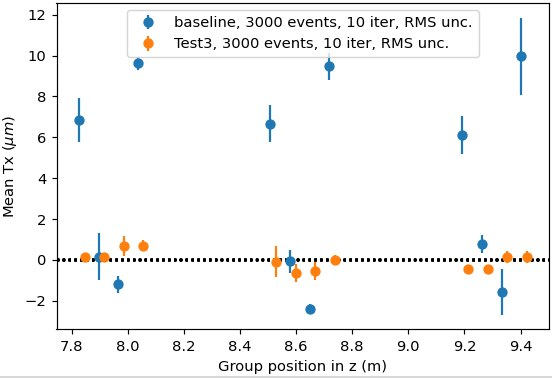
\includegraphics[width=\textwidth]{plots/renewed_plots/lxplus/4_10_a.jpeg}
    \caption{x-translation versus group position in z.}
    \label{fig:TxZ_1}
  \end{subfigure}
  \hfill
  \begin{subfigure}[b]{0.7\textwidth}
    \centering
    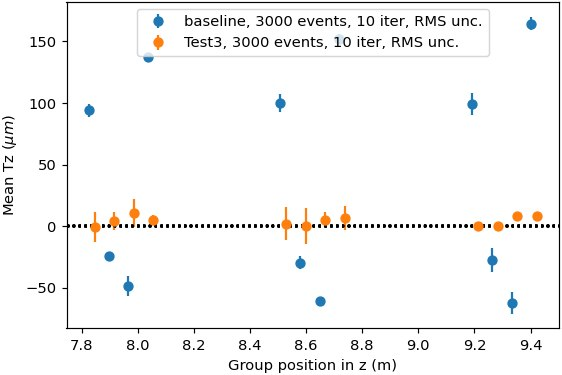
\includegraphics[width=\textwidth]{plots/renewed_plots/lxplus/4_10_b.jpeg}
    \caption{z-translation versus group position in z.}
    \label{fig:TxZ_2}
  \end{subfigure}
  \caption{"Test3" configuration (orange) plotted versus baseline configuration (blue) for 1000 events.}
  \label{fig:TxZ}
\end{figure}

Here the last four C-frame constraints have rotational degrees of freedom added.
Looking at \ref{fig:TxZ_1} each station has a quite low movement in x-direction comparing to the previous configurations. In the last station, the first two layers the C-side and A-side are exactly where they should be inside the detector since the RMS is very close to zero. The last two layers only show a small uncertainty. In station
two the X-layers are separating from the stereolayers. The X-layers also have a noticable RMS uncertainty. In this configuration the degrees of freedom are chose in a way for the alignment to either use them as two pairs of cartesian coordinates (Tx Tz, and Rx Rz) or interpret them as two pairs of polar coordinates (Tx Rz and Tz Rx).
This and also the reduction in constraints seemed to help the alignment in terms of x-translation, not so much regarding z-translation. Also this plot only shows the alignment for 1000 events and 10 iterations but overall an improvement was achieved
when it comes to constructing a good configuration.

The next configurations are called "config5" (blue) and "config5 Rz" (orange). The plots showing the translations are shown in figure \ref{fig:config5_tra} and the rotations are shown in figure \ref{fig:config5_rot}.
The blue measurement has the same constraints as "Test3" with an added back C-frame constraint:
\begin{lstlisting}[language=Python]
  constraints.append("back_C_frame_T3 : FT/T3/Layer(V|X2) : Tx Tz")
\end{lstlisting}

The orange measurement has a similar constraint added with Rz added to the DoFs inside the constraint:
\begin{lstlisting}[language=Python]
  constraints.append("back_C_frame_T3 : FT/T3/Layer(V|X2) : Tx Tz Rz")
\end{lstlisting}

Comparing just these two configurations, regarding $Tx$ there is not a big difference.
The last station has a little more separation in "config5 Rz", station 2 shows roughly the same performance and station one is also more split, in total approximately
$\SI{0.5}{\micro\metre}$. The overall z-translation regressed by a small amount in every station while the layer spearation in station 3 improved.
It can be seen, that both X-layers in T2 in the x-translation plot have a quite large RMS uncertainty which means the A-side and the C-side in the X-layers are quite far apart but the mean is right around 0. That is expected since the constraint added only brings the mean of the layer to 0. In future analyses new constraints will be added to bring the sides together.
% config 5
\begin{figure}
  \centering
  \begin{subfigure}[b]{0.48\textwidth}
    \centering
    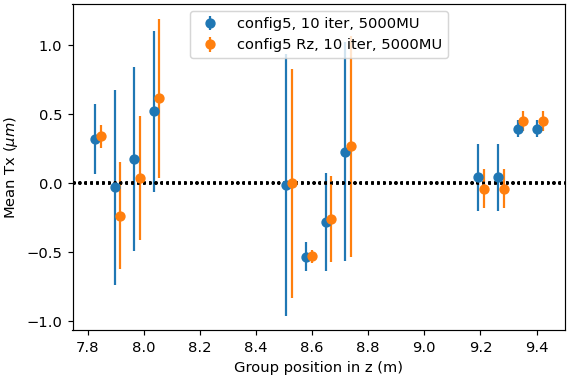
\includegraphics[width=\textwidth]{plots/renewed_plots/Tx_config5.png}
    \caption{x-translation versus group position in z.}
    \label{fig:config5_Tx}
  \end{subfigure}
  \hfill
  \begin{subfigure}[b]{0.48\textwidth}
    \centering
    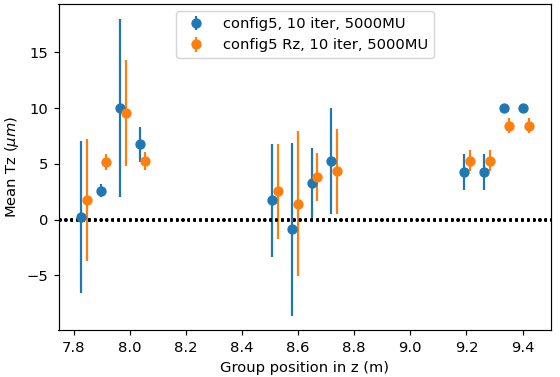
\includegraphics[width=\textwidth]{plots/renewed_plots/Tz_config5.png}
    \caption{z-translation versus group position in z.}
    \label{fig:config5_Tz}
  \end{subfigure}
  \caption{"config5" configurations (blue) plotted versus "config5 Rz" configuration (orange) for 5000 events.}
  \label{fig:config5_tra}
\end{figure}

Rotations around $x$ will not be further analysed because it does not have a huge impact on the alignment quality and is also very well aligned. In $Rz$ a noticable gap
between the two measurements can be seen. This is a result from the added $Rz$ constraint on the last two layers.
The constraints used should result in a rotation smaller than what is seen in figure \ref{fig:config5_Rz}.
A possible cause for that can be a bias inside the SciFi hit clusters and will be discussed later in section \ref{sec:clusterbias}.

\begin{figure}
  \centering
  \begin{subfigure}[b]{0.48\textwidth}
    \centering
    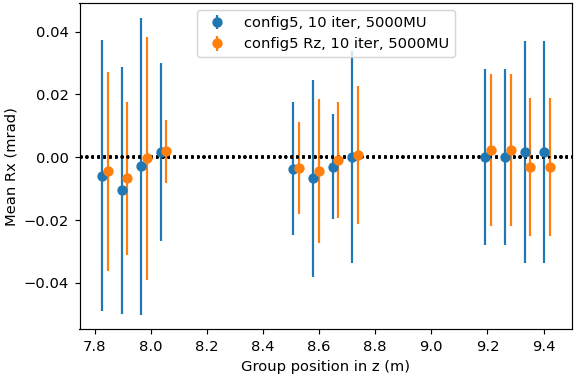
\includegraphics[width=\textwidth]{plots/renewed_plots/Rx_config5.png}
    \caption{x-rotation versus group position in z.}
    \label{fig:config5_Rx}
  \end{subfigure}
  \hfill
  \begin{subfigure}[b]{0.48\textwidth}
    \centering
    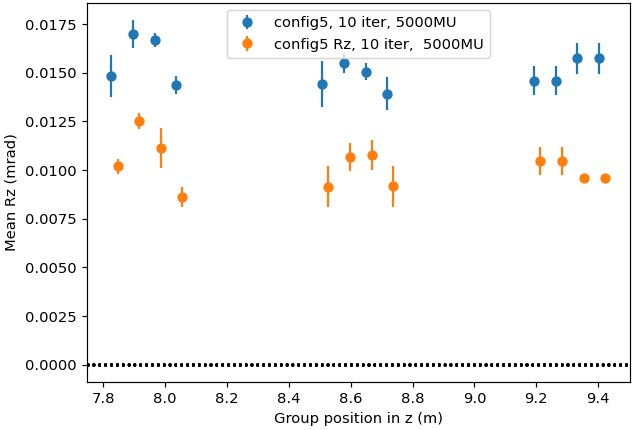
\includegraphics[width=\textwidth]{plots/renewed_plots/Rz_config5.png}
    \caption{z-rotation versus group position in z.}
    \label{fig:config5_Rz}
  \end{subfigure}
  \caption{"config5" configurations (blue) plotted versus "config5 Rz" configuration (orange) for 5000 events.}
  \label{fig:config5_rot}
\end{figure}

Regarding the goal to reduce the amount of rotation and translation in each station,
the result is a small improvement in $Rz$ of around $\SI{0.005}{\milli\radian}$ in every layer. $Rx$ is mostly unchanged as well as $Tx$.

Translation constraints as well as rotation constraints are not the only constraints tested. There are also scaling- and shearing constraints that were tested but seemed to have no major impact.

\section{chi2 tests and weak modes}
In this section, a $\chi^2$ analysis is performed in order to study the ``goodness'' of the alignment and determine the impact of potential weak modes also known as "correlated alignment parameters". There are several weak modes that could occur namely \textit{global translation}, \textit{shearing} and \textit{curvature bias}.
Weak modes are unaffected by the $\chi^2$ since the residuals do not change but they do however show in terms of the eigenvalues of track parameters.
The effect weak modes have on the alignment are biases regarding track parameters and late convergences.
There are different solutions that can be utilized to reduce the effect from weak modes such as
\begin{itemize}
  \item $\textbf{using other data-taking configurations like magnet off or mass plots \\for off-axis events}$
  \item $\textbf{utilizing other survey data sets}$
  \item $\textbf{using kinematic and vertex constraints}$
\end{itemize}\,.

Using magnet-off data can be helpfull as a comparison measurement since it can be utilized to constrain the curvature bias, which will not be element of this thesis but for future analyses.

\begin{figure}
  \centering
  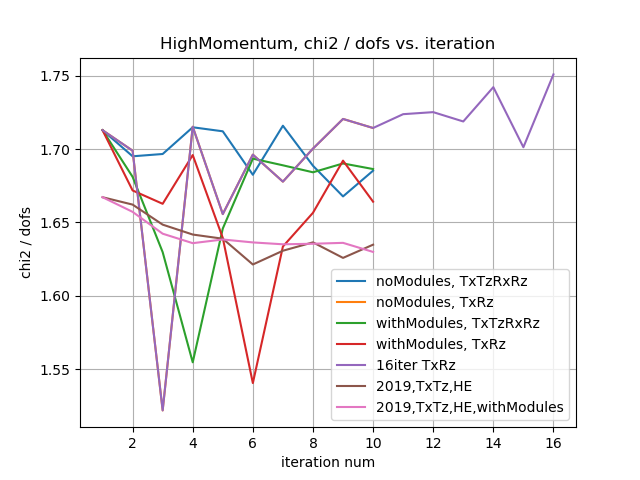
\includegraphics[width=0.8\textwidth]{plots/nov_19/Figure_2.png}
  \caption{$\chi^2 / dofs$ versus iteration number of different degrees of freedom, alignables and data samples.}
  \label{fig:fig2}
\end{figure}

The first test is the $\chi^2$-analysis for \textit{HighMomentumTTracks},
6500 events and 2020 MC data plotted versus the iteration number during the
alignment as shown in figure \ref{fig:fig2}.
This track selection was chosen because TTracks are mainly produced in secondary interactions and are identified by only having hits inside the T-stations as seen in figure \ref{fig:tracksel}.
\begin{figure}[!ht]
    \centering
    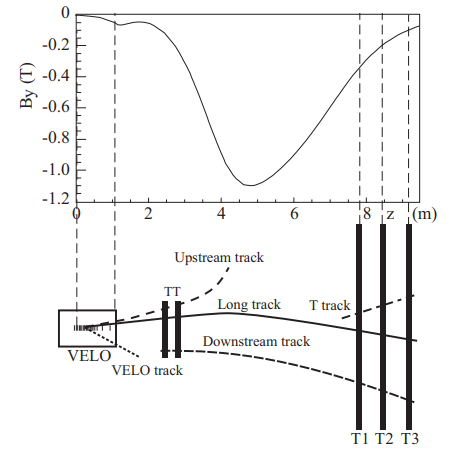
\includegraphics[width=0.8\textwidth]{plots/track_selection.png}
    \caption{An illustration of different track types as well as the main B-field component ($B_y$) as a function of the $z$ coordinate.}
    \label{fig:tracksel}
\end{figure}
Since the main B-field component is quite large inside the T-stations, \textit{HighMomentumTTracks} are especially useful for studies regarding magnet-off data because the difference between magnet-on and magnet-off is large.
These measurements are interesting to compare with studies regarding the curvature bias in future analyses.
In blue, stations and layers were aligned in $Tx$,
$Tz$, $Rx$ and $Rz$ with the constraints being used from "config5" from section \ref{sec:test_and_c5}. The orange
measurement is identical except for the degrees of freedom being only $Tx$ and $Rz$.
In green and red the same measurements as in blue and orange were performed with
the difference that that the modules are aligned as well.
The purple measurement is the only one which covers 16 iterations and is otherwise identical to the orange one. That is also why the orange measurement is not visible since it lies behind the purple one for the first 10 iterations.
the brown and pink measurements are done for simulated data with an older description of the detector geometry from 2019, and are otherwise identical to the orange and red measurement regarding constraints and alignable degrees of freedom.

The spiky behavior in this plot is not what we expected and this might be the result of weak modes since the convergence is quite bad in all of the 2020 data which can be seen by the $\chi^2 / dofs$ not steadily decreasing.
The 2019 measurements were performed as control measurements with and without
module alignment. Here a clear decrease in the $\chi^2 / dofs$ is visible. This
indicates that for the 2020 MC sample additional analysis must be performed to gain further knowledge about the MC data set since it shows some unclear findings.

The idea to test $Tx$, $Tz$, $Rx$ and $Rz$ versus only one translation and one
rotational degree of freedom was to analyse the effect regarding the convergence and the $\chi^2 / dofs$ itself. One could also argue that there was a quick convergence after three iterations when looking at the yellow measurement but something happened afterwards. This will be analysed in a future project.

In figure \ref{fig:chi2iter} a comparison between GoodLongTracks (left) and HighMomentumTTracks (right) for the same measurements was performed to to study the impact of different track selections. This shows, that the alignment quality for both track selections increases with the number of iterations.
The identical $\chi^2$ measurements for the HighMomentumTTracks were plotted against the number of tracks as seen in figure \ref{fig:chi2tracks} as an example.
A clear correlation between the $\chi^2 \ \text{dofs}$ and the number of tracks can be seen.

\begin{figure}
  \centering
  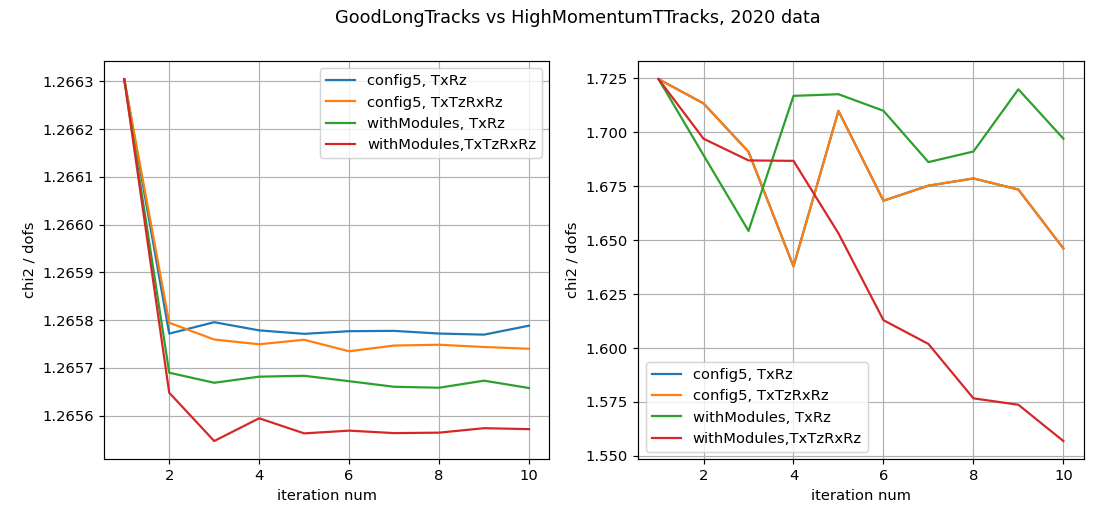
\includegraphics[width=0.8\textwidth]{plots/GL_HM_chi2_2020.png}
  \caption{$\chi^2$-test comparing GoodLongTracks (left) and HighMomentumTTracks (left) for different alignables and degrees of freedom.}
  \label{fig:chi2iter}
\end{figure}

\begin{figure}
  \centering
  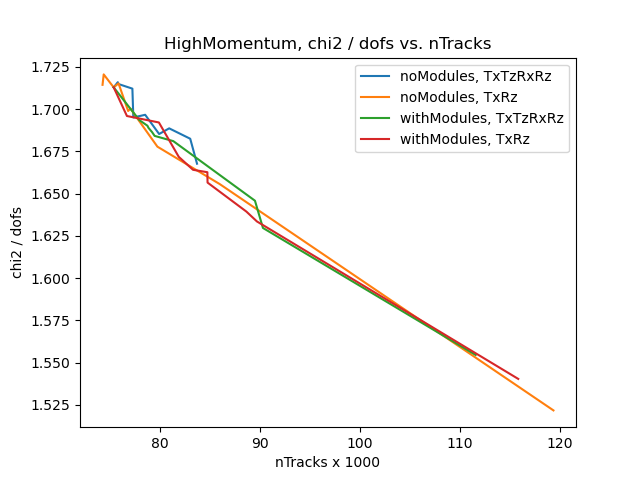
\includegraphics[width=0.8\textwidth]{plots/nov_21/chi2_vs_ntracks_all.png}
  \caption{$\chi^2$-test versus number of tracks of different degrees of freedom, alignables and data samples(redo with grid).}
  \label{fig:chi2tracks}
\end{figure}

\begin{figure}
  \centering
  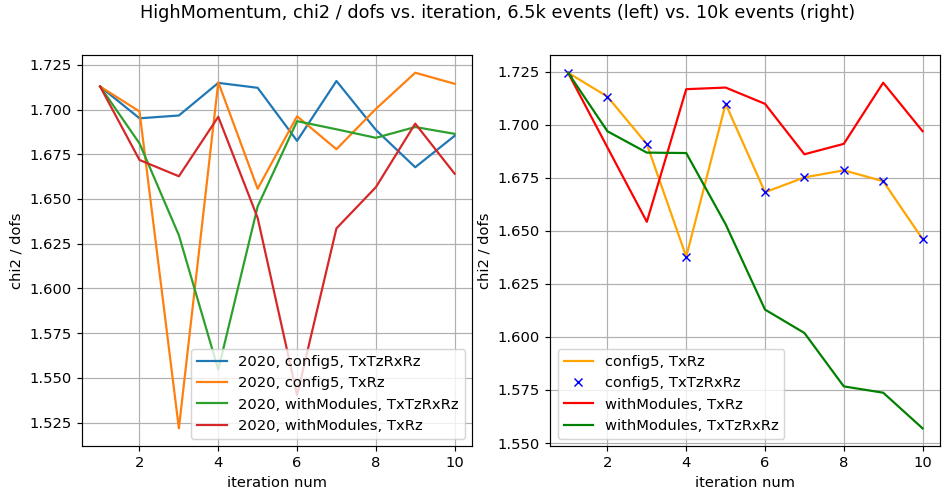
\includegraphics[width=\textwidth]{plots/renewed_plots/e5/4_17.png}
  \caption{$\chi^2 / \text{dofs}$ versus iteration number for different number of events.}
  \label{fig:chi2iterdec}
\end{figure}

In figure \ref{fig:chi2iterdec} a side-by-side view of the same $\chi^2$ measurement
is shown but for different number of events. Despite the different labels these are the same measurements, only the colors are switched around for red and green and also yellow and blue as a pair. The thing that strikes the eye is the steadily decrease in $\chi^2 / dofs$ in the red measurement. Unlike our first expectations that $Tx$ and $Rz$ are enough degrees of freedom to describe the system using additional degrees of freedom seemed to help the alignment.
Also, the blue measurement sits behind the orange which might be due to an
programming error.

In figure \ref{fig:chi2tracksdec} a consistency check for figure
\ref{fig:chi2iterdec} was performed. The number of tracks correlate well with
the $\chi^2 / \text{dofs}$.
% The blue measurement is missing again which seems to be a programming error.

\begin{figure}
  \centering
  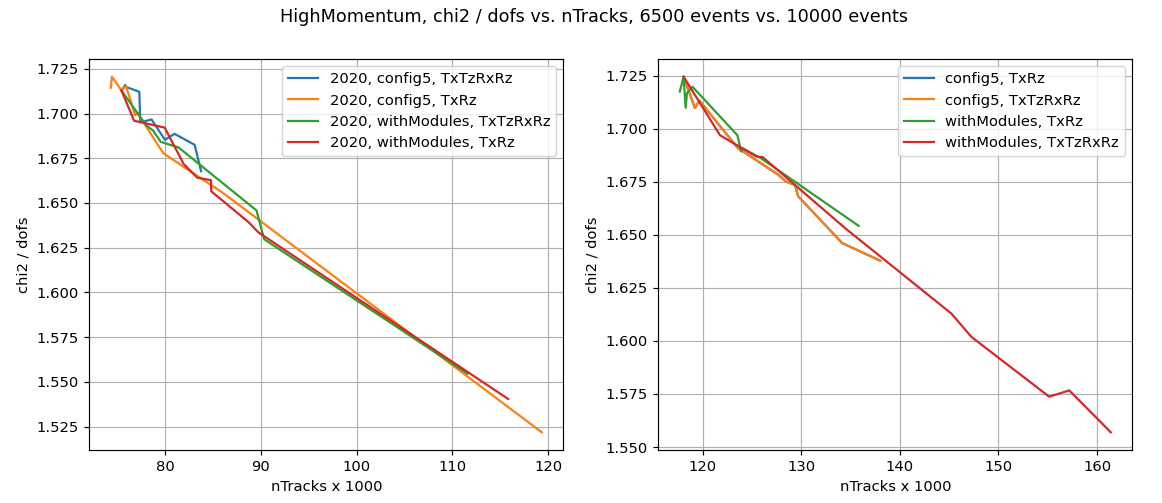
\includegraphics[width=\textwidth]{plots/LHCB_week_dec/chi2_vs_tracks_normal.png}
  \caption{$\chi^2 / \text{dofs}$ versus number of Tracks for 6500 events and 10000 events.}
  \label{fig:chi2tracksdec}
\end{figure}

We found out that the MC sample from 2020 using the newer detector geometry contains some aspects that require more tests for example the spikey behavior of the $\chi^2 / \text{dof}$. Figure \ref{fig:chi2iter} shows the same measurements for GoodLongTracks in comparison to HighMomentumTTracks which made it even more clear that the MC sample from 2020 is problematic. The GoodLongTracks shows an early convergence which is good. It also shows that aligning the modules of the SciFi instead of the stations and the half-layers is slightly better for the alignment performance. Hints of potential weak modes as well as the cluster bias could be the problem in the 2020 MC samples shown by the late convergence and the irregular behavior in the $\chi^2$ tests.

\section{impact of the cluster bias}
\label{sec:clusterbias}

To test the impact of the cluster bias, a momentary fix was found and implemented. The workaround was to add a scaling for the \textit{m\_airgap}\cite{gap} which is the gap between the modules as seen in figure \ref{fig:module_gap}.
As mentioned the cluster bias most certainly causes the shift in the rotation around $z$ for each layer so it does not reach 0.
Figure \ref{fig:cbhack_on_off} shows the impact of the cluster bias fix regarding the rotation around $z$.

\begin{figure}
  \centering
  \begin{subfigure}[b]{0.48\textwidth}
    \centering
    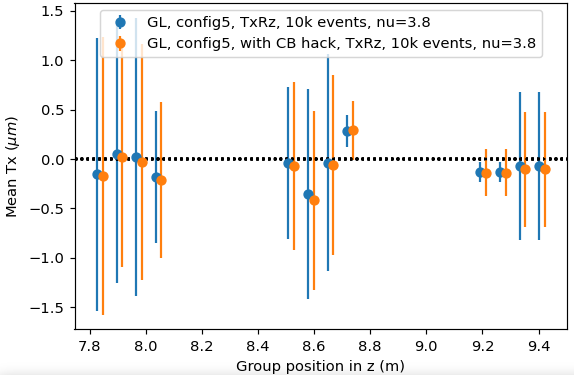
\includegraphics[width=\textwidth]{plots/renewed_plots/e5/4_19_3.png}
    \caption{plotted is the x-translation versus the group position in $z$.}
    \label{fig:cbTxlow}
  \end{subfigure}
  \hfill
  \begin{subfigure}[b]{0.48\textwidth}
    \centering
    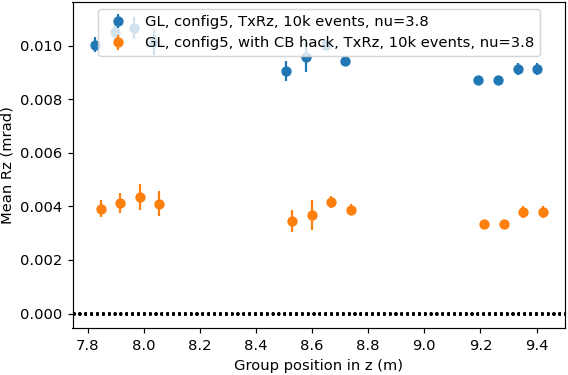
\includegraphics[width=\textwidth]{plots/renewed_plots/e5/4_19_4.png}
    \caption{plotted is the rotation around $z$ versus the group position in $z$.}
    \label{fig:cbRzlow}
  \end{subfigure}
  \caption{Impact of the cluster bias for the lower luminosity sample plotted for $z$-rotation and $x$-translation against the group position in $z$. GoodLongTracks were used with "config5" and 5000 events for 10 iterations.}
  \label{fig:cblow}
\end{figure}

\begin{figure}
  \centering
  \begin{subfigure}[b]{0.48\textwidth}
    \centering
    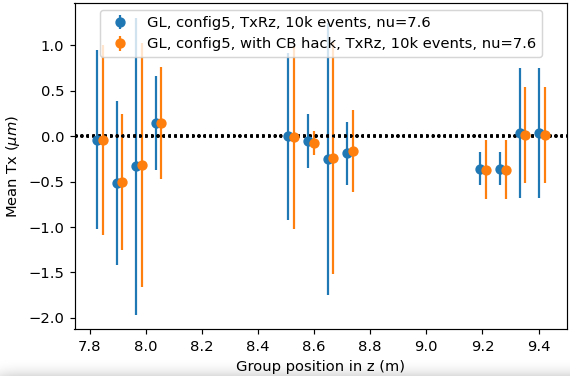
\includegraphics[width=\textwidth]{plots/renewed_plots/e5/4_19_1.png}
    \caption{plotted is the x-translation versus the group position in $z$.}
    \label{fig:cbTxlow}
  \end{subfigure}
  \hfill
  \begin{subfigure}[b]{0.48\textwidth}
    \centering
    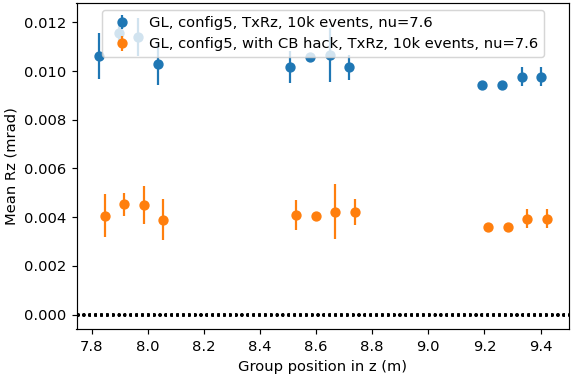
\includegraphics[width=\textwidth]{plots/renewed_plots/e5/4_19_2.png}
    \caption{plotted is the rotation around $z$ versus the group position in $z$.}
    \label{fig:cbRzlow}
  \end{subfigure}
  \caption{Impact of the cluster bias for the normal luminosity sample plotted for $z$-rotation and $x$-translation against the group position in $z$. GoodLongTracks were used with "config5" and 5000 events for 10 iterations.}
  \label{fig:cbnormal}
\end{figure}

As we expected, the amount of rotation was reduced to about
$\SI{0.004}{\milli\radian}$ from the previous $\SI{0.01}{\milli\radian}$ which is more than a factor of 2 improvement. Because the rotation still does not reach zero, we know that this is not a true fix for the cluster bias, and further analysis will be needed to find the true source. That analysis is beyond the scope of this thesis.

\begin{figure}
    \centering
    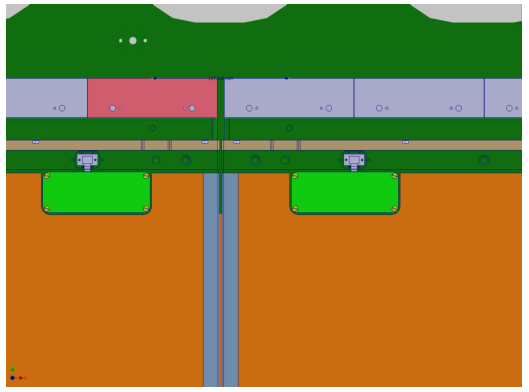
\includegraphics[width=0.8\textwidth]{plots/module_gap.png}
    \caption{Gap between the modules (orange). Borders (grey) are $\SI{6.8}{\milli\metre}$ apart from each other.}
    \label{fig:module_gap}
\end{figure}

\section{luminosity samples and chi2}
In order to get a clearer view of the difference in alignment quality, coming from the difference in luminosity during the ramp-up phase and the data taking phase, samples of different luminosities are looked at.
Comparing two samples, one with a "ramp-up" luminosity with a parameter $\nu = 3.8$ also referred to as "low luminosity" and one for the luminosity used during the data taking
with $\nu = 7.6$, called "normal luminosity".
The $\chi^2 / dofs$ of these samples is plotted versus the iteration number \ref{fig:chi2iter_lumi_normal} and the number of tracks\ref{fig:chi2tracks_lumi_normal}.

in figure \ref{fig:chi2iter_lumi_normal} we see the expected convergence after iteration three and a quite low $\chi^2 / dofs$ of around $\num{1.28595}$ for the normal luminosity sample
and $\num{1.3067}$ for the low luminosity sample.

\begin{figure}
  \centering
  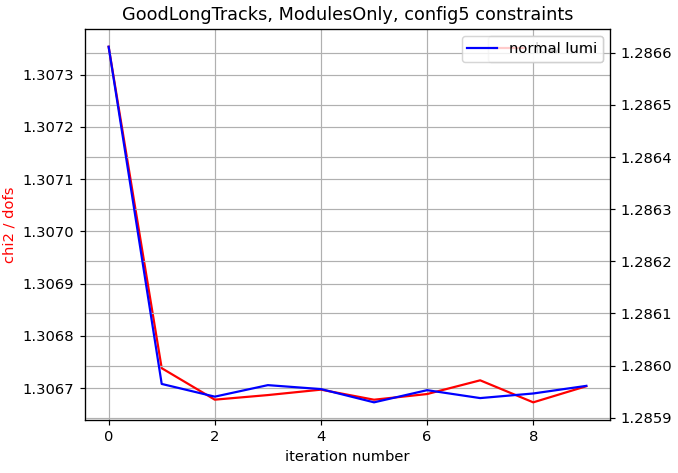
\includegraphics[width=0.8\textwidth]{plots/renewed_plots/modules_chi2_c5.png}
  \caption{compare different luminosities and plot $\chi^2$ versus iteration number.}
  \label{fig:chi2iter_lumi_normal}
\end{figure}

\begin{figure}
  \centering
  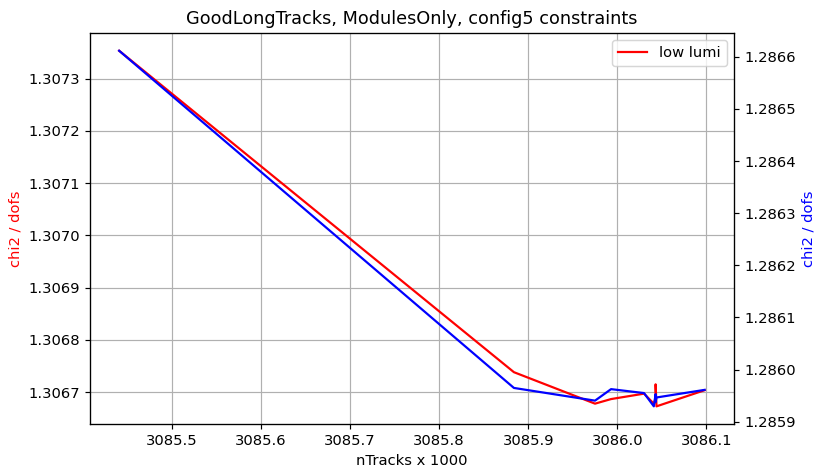
\includegraphics[width=0.8\textwidth]{plots/jan_17_2022/chi2_tracks_modulesOnly.png}
  \caption{compare different luminosities and plot $\chi^2$ versus number of tracks as a measurement for weak modes and alignment.}
  \label{fig:chi2tracks_lumi_normal}
\end{figure}

This short study shows, that the difference in alignment quality coming from different luminosities is small, which can be seen in the difference in $\chi^2 / \text{dofs}$. For both samples the convergence happened early, which is expected.

Now that we know that the cluster bias can be reduced we take a closer look at samples of different luminosities since the LHC will not be operated at the maximum luminosity from the start, there is also the ramp up phase where the luminosity will be lower.

Since we want to know what the shifts in rotation and translation will look like when the cluster bias is fixed we will keep the fix active for the next studies.
Figure \ref{fig:lumi_low_normal_hack_on} shows the difference between a sample with ramp-up luminosity and a sample with the luminosity during the measurement phase.
We see, that the layer separation is much more prominent in station 1 and 3 for the higher luminosity sample but slightly better behaved in station 2 when looking at x-translation.
Regarding the z-rotation, the lower luminosity sample as slightly lower rotational shifts.
The difference is so minute that it can be safely disregarded.

\begin{figure}
  \centering
  \begin{subfigure}[b]{0.48\textwidth}
    \centering
    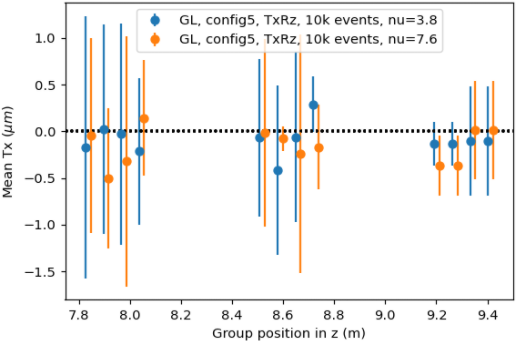
\includegraphics[width=\textwidth]{plots/jan_24_2022/tx_low_normal.png}
    \caption{plotted is the x-translation versus the group position in $z$.}
    \label{fig:compare_tx}
  \end{subfigure}
  \hfill
  \begin{subfigure}[b]{0.48\textwidth}
    \centering
    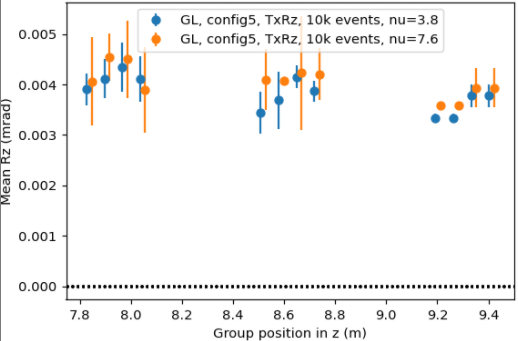
\includegraphics[width=\textwidth]{plots/jan_24_2022/rz_low_normal.png}
    \caption{plotted is the rotation around $z$ versus the group position in $z$.}
    \label{fig:compare_rz}
  \end{subfigure}
  \caption{Plotting the difference in $x$-translation and rotation around $z$ for low and normal luminosity sample for 10000 events and 10 iterations used. For this, the cluster bias fix is active.}
  \label{fig:lumi_low_normal_hack_on}
\end{figure}

With that, we tested if there is a noticable difference in the $\frac{\chi^2}{\text{dof}}$
and the result is shown in figure \ref{fig:GL_lumi_low_normal_hack_on}.

\begin{figure}
  \centering
  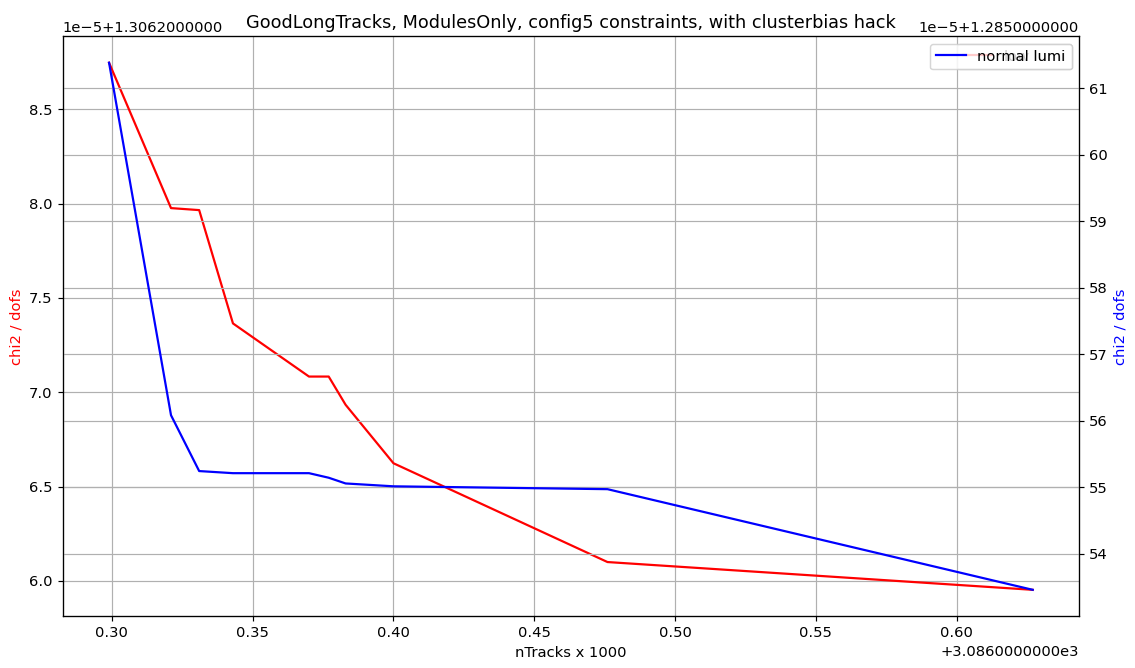
\includegraphics[width=0.8\textwidth]{plots/feb_2_2022/GL_modules_c5_cb_hackactive_low_normal_lumi.png}
  \caption{GoodLong tracks for module alignment and config 5 active. also the clusterbias fix is active comparing low and normal luminosity.}
  \label{fig:GL_lumi_low_normal_hack_on}
\end{figure}

\begin{figure}
  \centering
  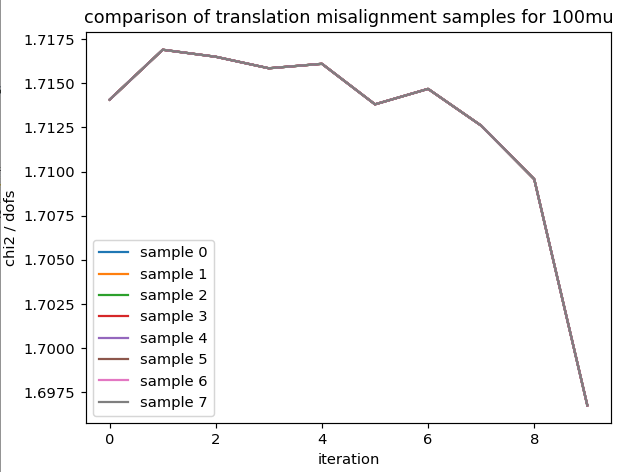
\includegraphics[width=0.8\textwidth]{plots/feb_6_2022/100mu_misalignment_samples_compared.png}
  \caption{100mu translation misalignment comparison for different misalignment samples.}
  \label{fig:100muT}
\end{figure}

Now, since the alignment works quite good with the current configuration we
tested how translation misalignment effects the convergence by looking at the
$\chi^2$, portrayed in figure \ref{fig:100muT}. For this figure, eight different samples of $\SI{100}{\micro\metre}$ module translation misalignment over all translatory
degrees of freedom. The idea behind using different samples is to reduce errors
from biased samples. The plot shows the total $\chi^2$ over degrees of freedom
plotted against the number of iterations. We see no visible difference regarding
the total $\chi^2$ between the samples which is good.
Also, the total $\chi^2$ decreases with an increasing number of iterations
during the alignment.

\begin{figure}
  \centering
  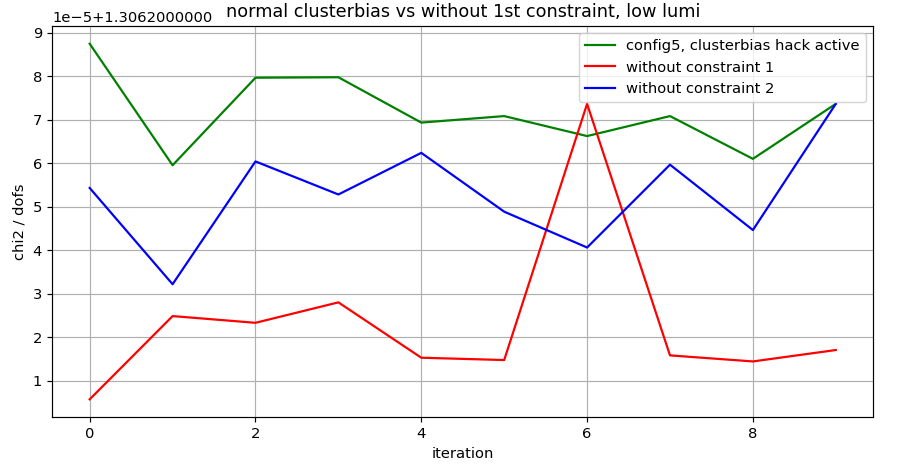
\includegraphics[width=0.8\textwidth]{plots/feb_6_2022/low_lumi_removed_constraints_vs_normal.png}
  \caption{impact of removing constraints from exisiting studies regarding chi2.}
  \label{fig:removeConst}
\end{figure}

We do want the least amount of constraints in the system so we also tested
the consequences of removing constraints from "config5".
The results are shown in figure \ref{fig:removeConst}.
The green curve shows the base configuration for comparison and in red the removal of the backlayer constraint in station 3 is shown. The blue curve shows the alignment results without the C-frame constraints.
The data samples used were from 2020 with the normal luminosity and an active clusterbias fix.
The selected track types are \textit{HighMomentumTTracks} for 10000 events.
On the one hand we see an improvement in $\chi^2 / \text{dof}$ when removing these constraints individually even if it is only on a very small scale of $\num{1e-5}$. On the
other hand we see that the $\chi^2 / \text{dof}$ after the last iteration is the same for the base config and for the blue measurement. The constraint removed in the red measurement seems to have the most impact from what was tested but the peak in iteration 6 has no logical
explanation. Additional analysis regarding constraint removal will be done in the future to analyse this phenomenon further.
Also the behavior of the not decreasing $\chi^2 / \text{dof}$ requires more testing.
What can be taken from this is that the removal of some constraints will help
the alignment but the cause of some abnormalities require more testing.

\section{Tests with input misalignments}
\label{sec:misalignment}
\subsection{Translation misalignment}
\label{sec:misT}

In order to evaluate the performance of the alignment with a given configuration in Monte Carlo simulations, input misalignments are used.

Starting with translation misalignments for the configuration "config5 Rz". The input misalignment is a random gaussian generated distribution. The translation misalignment used were $\SI{0.001}{\micro\metre}$ and $\SI{200}{\micro\metre}$ in $Tx$, $Ty$ and $Tz$ for the modules. We tested very small misalignment to be sure that this small deviation has no major impact on the alignment quality. $\SI{200}{\micro\metre}$ translation misalignment was tested since the position of a module within a C-frame is known within $\SI{200}{\micro\metre}$.

The differences between the misaligned "config5 Rz" and the normal configuration plotted for each of the used degrees of freedom are shown in the following figures \ref{fig:mis_Tx} to \ref{fig:mis_Rz}.

\begin{figure}
  \centering
  \begin{subfigure}[b]{0.48\textwidth}
    \centering
    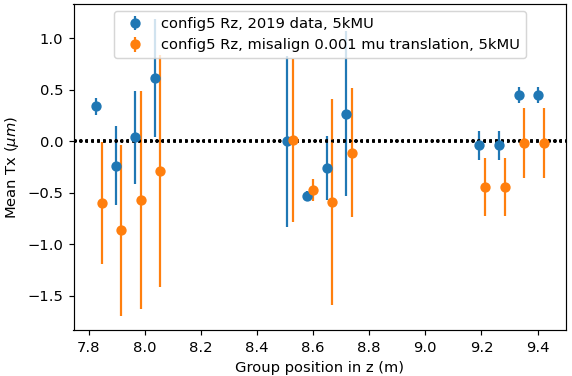
\includegraphics[width=\textwidth]{plots/misalign_transl/Tx_0001mu_translation.png}
    \caption{$\SI{0.001}{\micro\metre}$ module translation misalignment.}
    \label{fig:00001Tx}
  \end{subfigure}
  \hfill
  \begin{subfigure}[b]{0.48\textwidth}
    \centering
    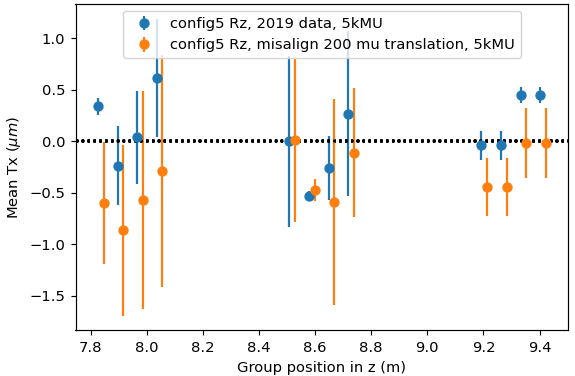
\includegraphics[width=\textwidth]{plots/misalign_transl/Tx_200mu_translation.png}
    \caption{$\SI{200}{\micro\metre}$ module translation misalignment.}
    \label{fig:200Tx}
  \end{subfigure}
  \caption{Plotted is configuration "config5 Rz" (blue) versus itself with translation misalignments (orange). The alignment run used 10 iterations and 5000 events. The translation in $x$ is plotted against the group position in $z$.}
  \label{fig:mis_Tx}
\end{figure}

\begin{figure}
  \centering
  \begin{subfigure}[b]{0.48\textwidth}
    \centering
    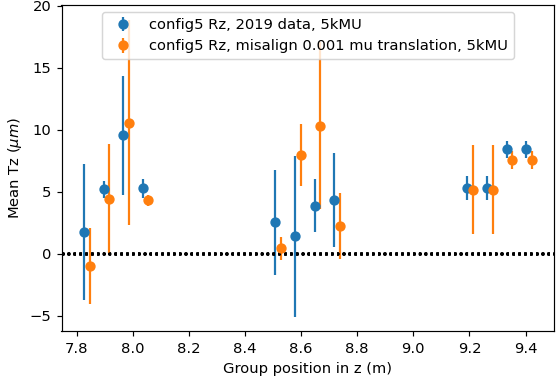
\includegraphics[width=\textwidth]{plots/misalign_transl/Tz_0001mu_translation.png}
    \caption{$\SI{0.001}{\micro\metre}$ module translation misalignment.}
    \label{fig:00001Tz}
  \end{subfigure}
  \hfill
  \begin{subfigure}[b]{0.48\textwidth}
    \centering
    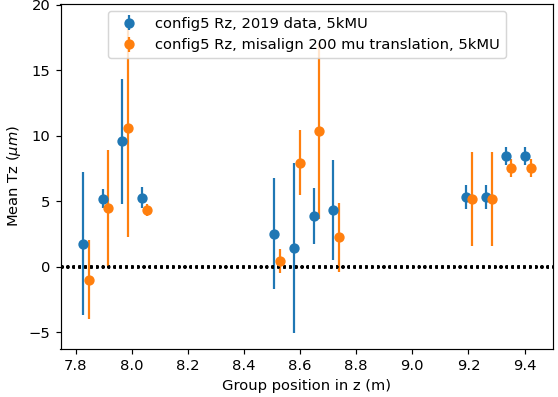
\includegraphics[width=\textwidth]{plots/misalign_transl/Tz_200mu_translation.png}
    \caption{$\SI{200}{\micro\metre}$ module translation misalignment.}
    \label{fig:200Tz}
  \end{subfigure}
  \caption{Plotted is configuration "config5 Rz" (blue) versus itself with translation misalignments (orange). The alignment run used 10 iterations and 5000 events. The translation in $z$ is plotted against the group position in $z$.}
  \label{fig:mis_Tz}
\end{figure}

\begin{figure}
  \centering
  \begin{subfigure}[b]{0.48\textwidth}
    \centering
    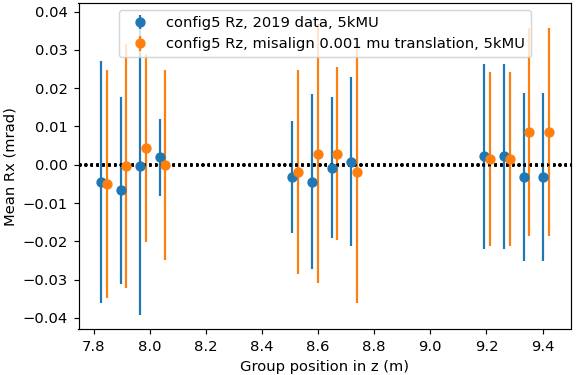
\includegraphics[width=\textwidth]{plots/misalign_transl/Rx_0001mu_translation.png}
    \caption{$\SI{0.001}{\micro\metre}$ module translation misalignment.}
    \label{fig:00001Rx}
  \end{subfigure}
  \hfill
  \begin{subfigure}[b]{0.48\textwidth}
    \centering
    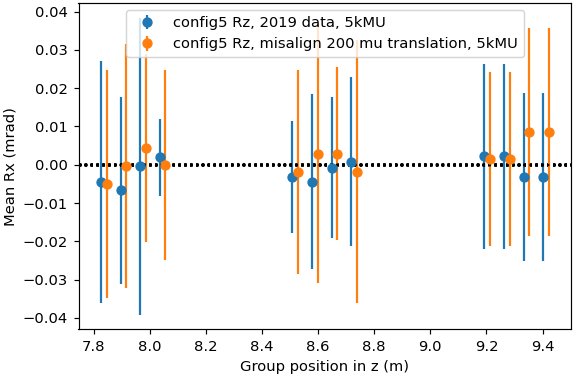
\includegraphics[width=\textwidth]{plots/misalign_transl/Rx_200mu_translation.png}
    \caption{$\SI{200}{\micro\metre}$ module translation misalignment.}
    \label{fig:200Rx}
  \end{subfigure}
  \caption{Plotted is configuration "config5 Rz" (blue) versus itself with translation misalignments (orange). The alignment run used 10 iterations and 5000 events. The rotation around $x$ is plotted against the group position in $z$.}
  \label{fig:mis_Rx}
\end{figure}

\begin{figure}
  \centering
  \begin{subfigure}[b]{0.48\textwidth}
    \centering
    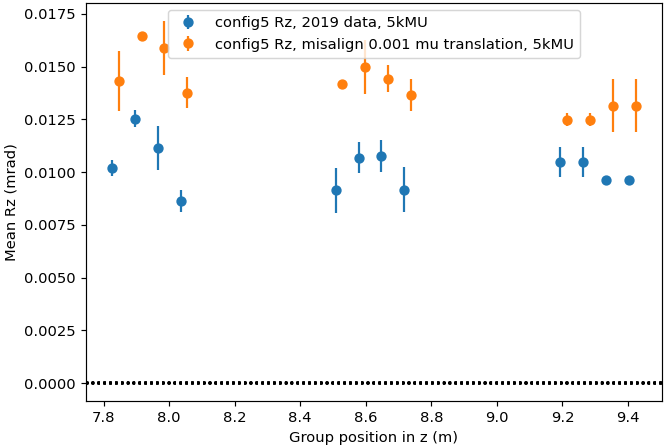
\includegraphics[width=\textwidth]{plots/misalign_transl/Rz_0001mu_translation.png}
    \caption{$\SI{0.001}{\micro\metre}$ module translation misalignment.}
    \label{fig:00001Rz}
  \end{subfigure}
  \hfill
  \begin{subfigure}[b]{0.48\textwidth}
    \centering
    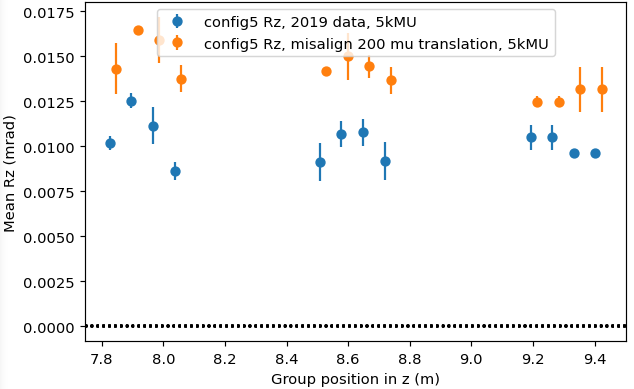
\includegraphics[width=\textwidth]{plots/misalign_transl/Rz_200mu_translation.png}
    \caption{$\SI{200}{\micro\metre}$ module translation misalignment.}
    \label{fig:200Rz}
  \end{subfigure}
  \caption{Plotted is configuration "config5 Rz" (blue) versus itself with translation misalignments (orange). The alignment run used 10 iterations and 5000 events. The rotation around $z$ is plotted against the group position in $z$.}
  \label{fig:mis_Rz}
\end{figure}

It becomes clear, that the alignment for both amounts of input misalignment worked equally good. There is a little discrepancy to the non-misaligned configuration but the differences are small enough to be negligible.
The chosen configuration is therefore capable of handling misalignments of $\SI{200}{\micro\metre}$.

\subsection{Rotation misalignment}
\label{sec:misR}

Regarding rotation misalignments, the amount of misalignment chosen was based on the scale of $Rz$.
The two input misalignments shown in the following plots are $\SI{0.01}{\milli\radian}$ and $\SI{0.1}{\milli\radian}$ gaussian generated distributions. The former is roughly the scale of $z$-rotation wheras the latter is scaled up by a factor of ten.

% if i have time and lxplus lets me use my python scripts i will make them new. otherwise this is the comparisons we are using

\begin{figure}
  \centering
  \begin{subfigure}[b]{0.48\textwidth}
    \centering
    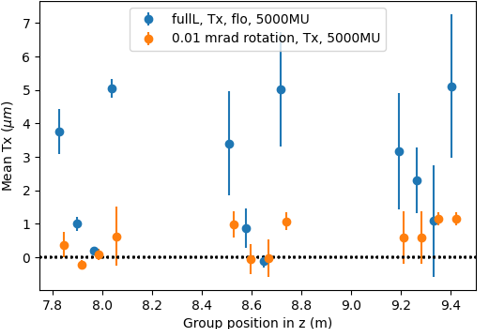
\includegraphics[width=\textwidth]{plots/misalign_rota/001_rot_Tx.png}
    \caption{$\SI{0.01}{\milli\radian}$ module rotation misalignment.}
    \label{fig:001Tx}
  \end{subfigure}
  \hfill
  \begin{subfigure}[b]{0.48\textwidth}
    \centering
    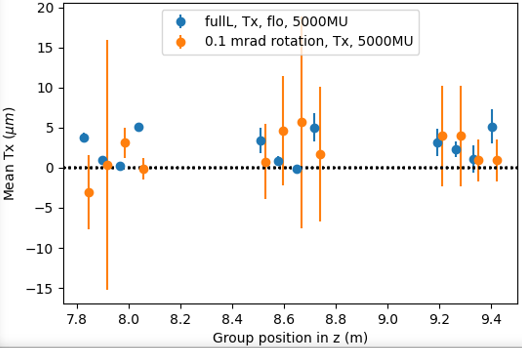
\includegraphics[width=\textwidth]{plots/misalign_rota/01_rot_Tx.png}
    \caption{$\SI{0.1}{\milli\radian}$ module rotation misalignment.}
    \label{fig:01Tx}
  \end{subfigure}
  \caption{Plotted is configuration "baseline" (blue) versus "config5 Rz" with translation misalignments (orange). The alignment run used 10 iterations and 5000 events. The translation in $x$ is plotted against the group position in $z$.}
  \label{fig:mis_rot_Tx}
\end{figure}

\begin{figure}
  \centering
  \begin{subfigure}[b]{0.48\textwidth}
    \centering
    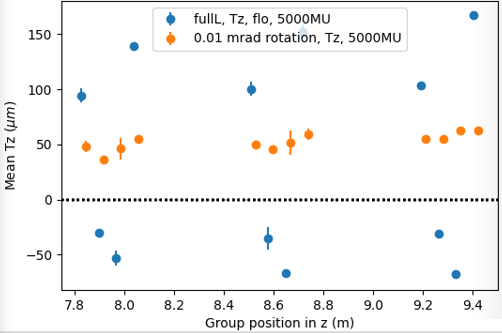
\includegraphics[width=\textwidth]{plots/misalign_rota/001_rot_Tz.png}
    \caption{$\SI{0.01}{\milli\radian}$ module rotation misalignment.}
    \label{fig:001Tz}
  \end{subfigure}
  \hfill
  \begin{subfigure}[b]{0.48\textwidth}
    \centering
    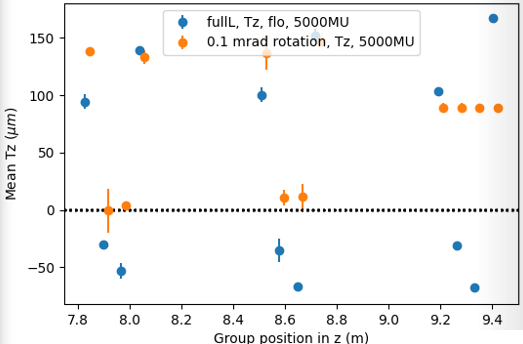
\includegraphics[width=\textwidth]{plots/misalign_rota/01_rot_Tz.png}
    \caption{$\SI{0.1}{\milli\radian}$ module rotation misalignment.}
    \label{fig:01Tz}
  \end{subfigure}
  \caption{Plotted is configuration "baseline" (blue) versus "config5 Rz" with translation misalignments (orange). The alignment run used 10 iterations and 5000 events. The translation in $z$ is plotted against the group position in $z$.}
  \label{fig:mis_rot_Tx}
\end{figure}

\begin{figure}
  \centering
  \begin{subfigure}[b]{0.48\textwidth}
    \centering
    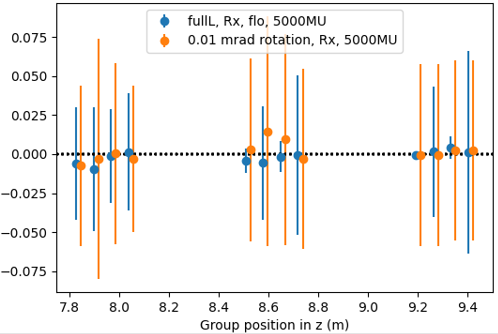
\includegraphics[width=\textwidth]{plots/misalign_rota/001_rot_Rx.png}
    \caption{$\SI{0.01}{\milli\radian}$ module rotation misalignment.}
    \label{fig:001Rx}
  \end{subfigure}
  \hfill
  \begin{subfigure}[b]{0.48\textwidth}
    \centering
    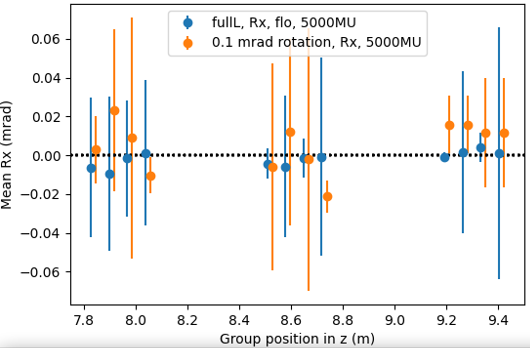
\includegraphics[width=\textwidth]{plots/misalign_rota/01_rot_Rx.png}
    \caption{$\SI{0.1}{\milli\radian}$ module rotation misalignment.}
    \label{fig:01Rx}
  \end{subfigure}
  \caption{Plotted is configuration "baseline" (blue) versus "config5 Rz" with translation misalignments (orange). The alignment run used 10 iterations and 5000 events. The rotation around $x$ is plotted against the group position in $z$.}
  \label{fig:mis_rot_Rx}
\end{figure}

\begin{figure}
  \centering
  \begin{subfigure}[b]{0.48\textwidth}
    \centering
    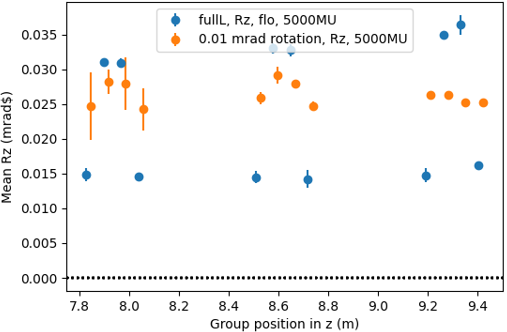
\includegraphics[width=\textwidth]{plots/misalign_rota/001_rot_Rz.png}
    \caption{$\SI{0.01}{\milli\radian}$ module rotation misalignment.}
    \label{fig:001Rz}
  \end{subfigure}
  \hfill
  \begin{subfigure}[b]{0.48\textwidth}
    \centering
    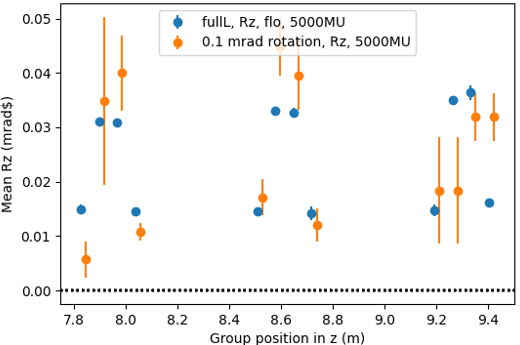
\includegraphics[width=\textwidth]{plots/misalign_rota/01_rot_Rz.png}
    \caption{$\SI{0.1}{\milli\radian}$ module rotation misalignment.}
    \label{fig:01Rz}
  \end{subfigure}
  \caption{Plotted is configuration "baseline" (blue) versus "config5 Rz" with translation misalignments (orange). The alignment run used 10 iterations and 5000 events. The rotation around $z$ is plotted against the group position in $z$.}
  \label{fig:mis_rot_Rz}
\end{figure}

It is clearly visible, that even a small rotation misalignment has an impact on the alignment quality. An input misalignment of $\SI{0.1}{\milli\radian}$ on the modules is enough to no longer be able to align the detector.
